% Created 2017-10-31 Tue 11:25
% Intended LaTeX compiler: pdflatex
\documentclass[11pt]{article}
\usepackage[utf8]{inputenc}
\usepackage[T1]{fontenc}
\usepackage{graphicx}
\usepackage{grffile}
\usepackage{longtable}
\usepackage{wrapfig}
\usepackage{rotating}
\usepackage[normalem]{ulem}
\usepackage{amsmath}
\usepackage{textcomp}
\usepackage{amssymb}
\usepackage{capt-of}
\usepackage{hyperref}
\usepackage{minted}
\usepackage{pdflscape}
\author{Willian Ver Valen Paiva}
\date{}
\title{Capstone Proposal}
\hypersetup{
 pdfauthor={Willian Ver Valen Paiva},
 pdftitle={Capstone Proposal},
 pdfkeywords={},
 pdfsubject={},
 pdfcreator={Emacs 27.0.50 (Org mode 9.1.1)}, 
 pdflang={English}}
\begin{document}

\maketitle

\section{Machine Learning Engineer Nanodegree}
\label{sec:org1223897}
\subsection{Domain Background}
\label{sec:org7c4259d}

For a long time work in facial recognition has being done and one of the key
points of this work is the face alignment as it poses its own challenge.
And the main tool used for the job is OpenCV which is used with DLIB to
recognize Facial landmarks.

The automatic recognition of landmarks is essential to be able to classify
facial expressions, or face tracking, face animation, and even 3D face
modeling.

For example to classify facial expressions it is necessary to classify
Facial Action Units also known as FACS \cite{ekman1977facial}, which in turn
needs a proper face alignment.

As one of my main projects today is to create a model capable to recognize
facial expression of pain, this subject comes to be perfect as it cover a
personal necessity and brings a good subject to work and learn.


\subsection{Problem Statement}
\label{sec:orgc813de3}
The problem of face alignment is among the most popular in the field of
computer vision and today we have many different implementations to
automatically recognize facial landmarks on images.
The most known is the Active Appearance Model (AAM)
\cite{edwards1998face,matthews2004active}.

But today we also some good results using Deep learning to achieve the
results for example the work done by Adrian Bulat on recognizing 3D facial
landmarks \cite{bulat2017far} that shows remarkable results it is implemented in torch.
a framework for \textbf{LUA}.

In resume to find an implementations on Tensorflow is not that easy. As most of the
works done on the subject is heavily dependent of DLIB to recognize the
landmarks. and as of today Tensorflow is a library that is on the rise and having such a
tool would be a plus and a entry point for more detailed facial expressions.

So for that reason I propose for this project to create a Deep Neural Network to
tackle such subject and have a model with better of equivalent performance of
the DLIB counter part on Tensorflow.

As the DLIB model has difficulty on recognizing points on faces by the side
view. 

The problem in question take a image as input (the format and details will be
discussed on the dataset section), and by using a regression model to
calculate the position of the face landmarks on the given image. 

\subsection{Dataset and Inputs}
\label{sec:org04b013a}

When looking for a data set for facial landmarks is possible to find many of
them example:

\begin{itemize}
\item AFLW \cite{sagonas2013300}
\item Cohn-Kanade AU-Coded Expression Database \cite{cohn1999cohn}
\item Affectiva-mit facial expression dataset (am-fed) \cite{mcduff2013affectiva}
\end{itemize}

But for this capstone project I propose to use the MUCT Face Database
\cite{Milborrow10}, this dataset consists of pictures (resolution 480x640) taken from 276 subjects
using 5 cameras in different angles (totalizing) an light conditions like the image below:

\begin{figure}[htbp]
\centering
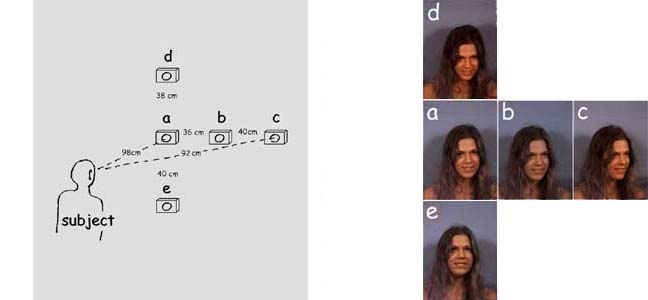
\includegraphics[width=.9\linewidth]{./images/muct-views-lores.jpg}
\caption{There is no images on the left but they cam be reproduced by mirroring the right side}
\end{figure}

Each picture is manually coded with 76 facial landmark like:
\begin{center}
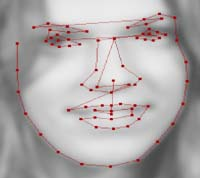
\includegraphics[width=.9\linewidth]{./images/landmarks.jpg}
\end{center}


The landmarks are saved in to 4 different file formats

\begin{itemize}
\item muct76.shape       shape file \cite{milborrow2009active}
\item muct76.rda         R data file (www.r-project.org/
\item muct76.csv         comma separated values
\item muct76-opencv.csv  comma separated values in OpenCV coords (0,0 at top left).
\end{itemize}


Note that the coordinate system in these files is the one used by
Stasm (i.e. the origin 0,0 is the center of the image, x increases as
you move right, y increases as you move up).  The exception is
muct76-opencv.csv, where the format is the "OpenCV format" (i.e. the
origin 0,0 is at the top left, x increases as you move left, y
increases as you move down).

Unavailable points are marked with coordinates 0,0 (regardless of the
coordinate system mentioned above).  "Unavailable points" are points
that are obscured by other facial features.  (This refers to landmarks
behind the nose or side of the face -- the position of such landmarks
cannot easily be estimated by human landmarkers -- in contrast, the
position of landmarks behind hair or glasses was estimated by the
landmarkers).  

So any points with the coordinates 0,0 should be ignored.  Unavailable
points appear only in camera views b and c.  Unless your software
knows how to deal with unavailable points, you should use only camera
views a, d, and e.

Note that subjects 247 and 248 are identical twins.


When talking about the train and testing split I will split the data into
train 70\% and test 30\% but it cannot be a random split as we have many images
of a same subject.
So to be sure the test set is well done the split has to be node at a subject
level so the same person cannot be found on test and train.

The choice of this dataset is made because it has a reasonable size to train
on personal computers and moreover it has large room for data augmentation
if necessary
The focus on using this data set is that it provides data
to have a better result when the face is in the side view.


The dataset is public available via github on the following link
\url{https://github.com/StephenMilborrow/muct}

\subsection{Solution Statement}
\label{sec:org3e1888b}

What I am hoping to achieve from this project is to have a pre trained model that is capable
of marking images properly with landmarks using a Tensorflow  backend, obtaining 
achieve results at least as good as the DLIB model, for that I will be using
our own Convolutional Neural Networks and pre-trained networks to find the best
result for the task.
as benchmark I will aim high for this project to to start I will create a
model based on the inceptionV3  and just change the final layer to a
regression and use it as the first result to compare the progress.
The main idea here is to create a model with 152 regression outputs giving
the respective X and Y of each point.

\subsection{Evaluation and Metrics}
\label{sec:org7ebac43}

As the problem consists on a regression model I believe that for the
evaluation of the results I could use the accuracy calculated by using the
regression functions Root Mean Squared Error. 

\subsection{Project Design}
\label{sec:org190fc9a}


To solve such a problem I will begin from preparing the data by doing a
proper split and assuring that the same subject cannot be fount on the train
and testing set, also some statistical on the data to be sure to have a fair
distribution of people of different sex, race, with/without glasses on both
sets.

Also gaining some insight on the data.

From that I will use the pre-trained inceptionV3 and create the benchmark
model for the project.

Once the environment is prepared the aim is to create many models until it
reaches a good result. 
As planned:

\begin{itemize}
\item create a CNN from scratch
\item use transfer leaning (inceptionV3, Resnet50, VGG16,\ldots{})
\end{itemize}

When creating my own CNN model i will be starting from the basic 5 Conv
layers followed by 3 dense layers (a bit like the AlexNet architecture) and from that work up the architecture test
and error.  

\begin{center}
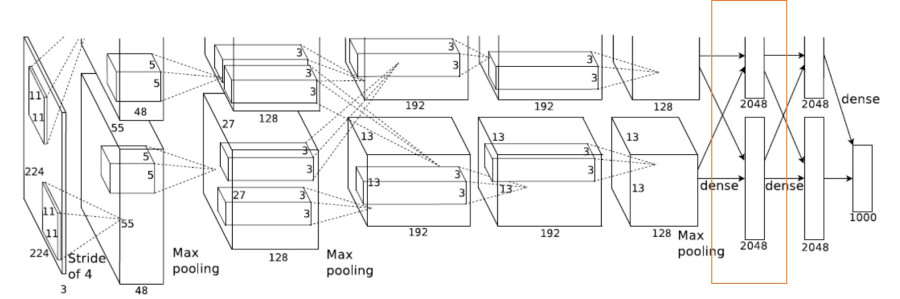
\includegraphics[width=.9\linewidth]{./images/alexnet6.jpg}
\end{center}

In case the transfer learning don't give good results another approach would
be go up on the pre-trained model and get more fine tuning.
By using the option include\(_{\text{top}}\) from keras and augment the number of layers
that will be trained. What would increase the time of training but give better results.

So for this capstone will be pushing the max i can to reach a best model at
the limit of computational power to train such models






\bibliographystyle{unsrt}
\bibliography{repport}
\end{document}